\documentclass[report.tex]{subfiles}

\begin{document}

\section{Exploratívna analýza}
\label{sec:explore}
V exploratívnej analýze sme sa zamerali na ukázanie relevantnosti dát, ktoré sme nazbierali a rovnako aj na vytvorenie si očakávaní od predikčného modelu. Teda po nazbieraní a uprataní dát sme hlavne riešili to, ako dané dáta budeme kombinovať a či niektoré z nich budú relevantné pre náš predikčný model.

\subsection{Náhľad do dát polls\_by\_election}
Hlavný dataset \verb*|data/polls_by_election.csv| obsahuje dáta, ktorý máme v pláne v upravenej verzii použiť na predikciu volebných výsledkov. Pre každú stranu dataset obsahuje posledných 12 prieskumov a výsledky volieb spolu s informáciami, či bola strana v parlamente, opozícii, alebo koalícii. Bolo by teda vhodné sa pozrieť na to, ako sa vyvíjali volebné prieskumy 12 mesiacov pred voľbami. Ak by sme našli jasné trendy, kedy strana postupne rastie v čase, chceli by sme očakávať od nášho modelu, že tento rast sa v ňom ukáže. 

Na ukážku sme si vybrali dáta z minuloročných volieb a rovnako sme vyfiltrovali strany, čo dosiahli v prieskumoch pred voľbami nenulový výsledok. 

\begin{figure}[!htbp]
    \centering
    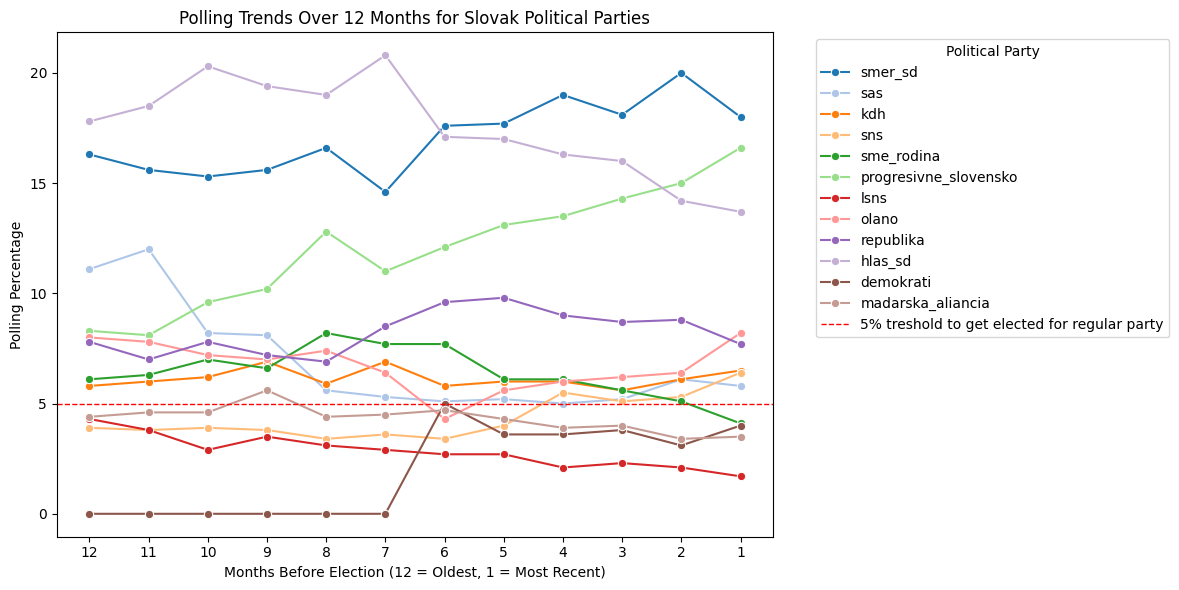
\includegraphics[width=\textwidth]{images_exploratory/Polls_without_result_2023.png}
    \caption{}
\end{figure}

Už môžeme pozorovať ako sa vyvíjali názory voličov pred voľbami, napríklad zrod strany Demokrati, mierny prepad Hlasu, či postupný nárast Progresívneho Slovenska. Pridanie výsledku vo voľbách by malo ešte väčšiu výpovednú hodnotu, keďže budeme vedieť zhodnotiť aj to, ako sa preferencie premietli už aj vo voľbách, a tak urobíme presne to.
\begin{figure}[H]
    \centering
    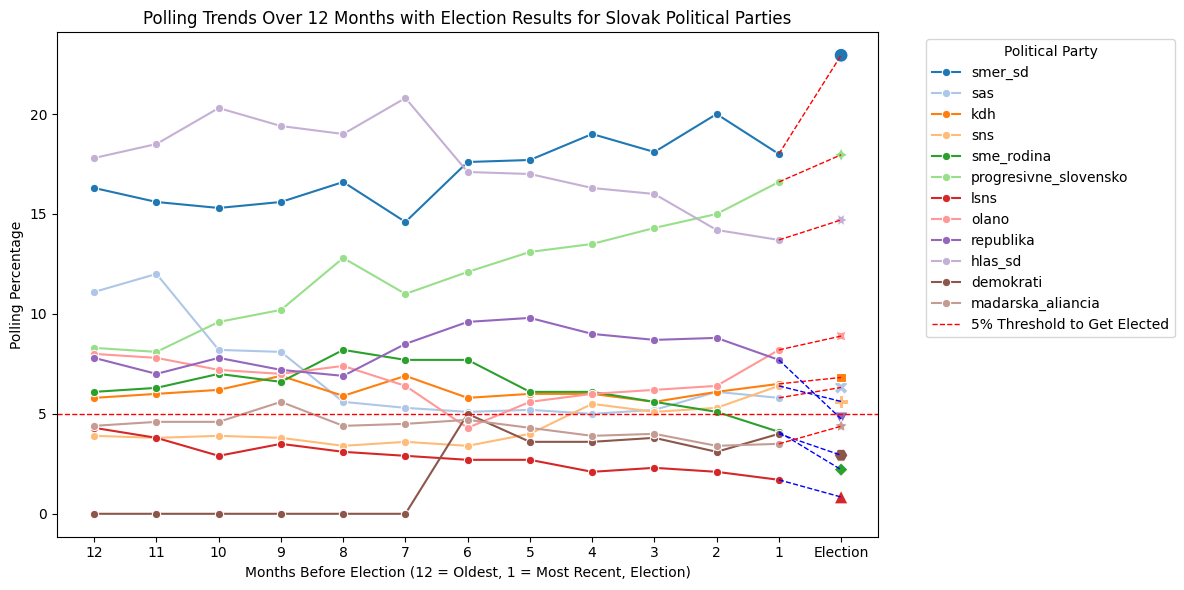
\includegraphics[width=\textwidth]{images_exploratory/Polls_with_result_2023.png}
    \caption{}
\end{figure}

Je jasné, že prieskumy zachytávajú realitu pred voľbami relatívne dobre, aj keď vidíme aj značné skoky pre určité strany. Avšak poradie toho ako strany dopadli vo voľbách sa skoro nezmenilo, až na výrazný prepad strany Republika.
Vidíme aj, že trendy v prieskumoch majú vplyv na to, ako strana dopadne vo voľbách. Aj tu sa nájdu výnimky, ako Hlas, ktorý niekoľko mesiacov pred voľbami padal, ale nakoniec dopadol lepšie, ako v posledných prieskumoch. Taktiež, ak sa niektoré strany dostali až pod hranicu zvoliteľnosti v prieskumoch, často ju už neprekonali. Voliči majú prirodzený strach, že im prepadne hlas, a tak práve takýto výsledok v prieskumoch môže veľmi ublížiť strane.

Toto bol pohľad len na najnedávnejšie voľby, ale ako vyzerali aj tie predtým?

\begin{figure}[H]
    \centering
    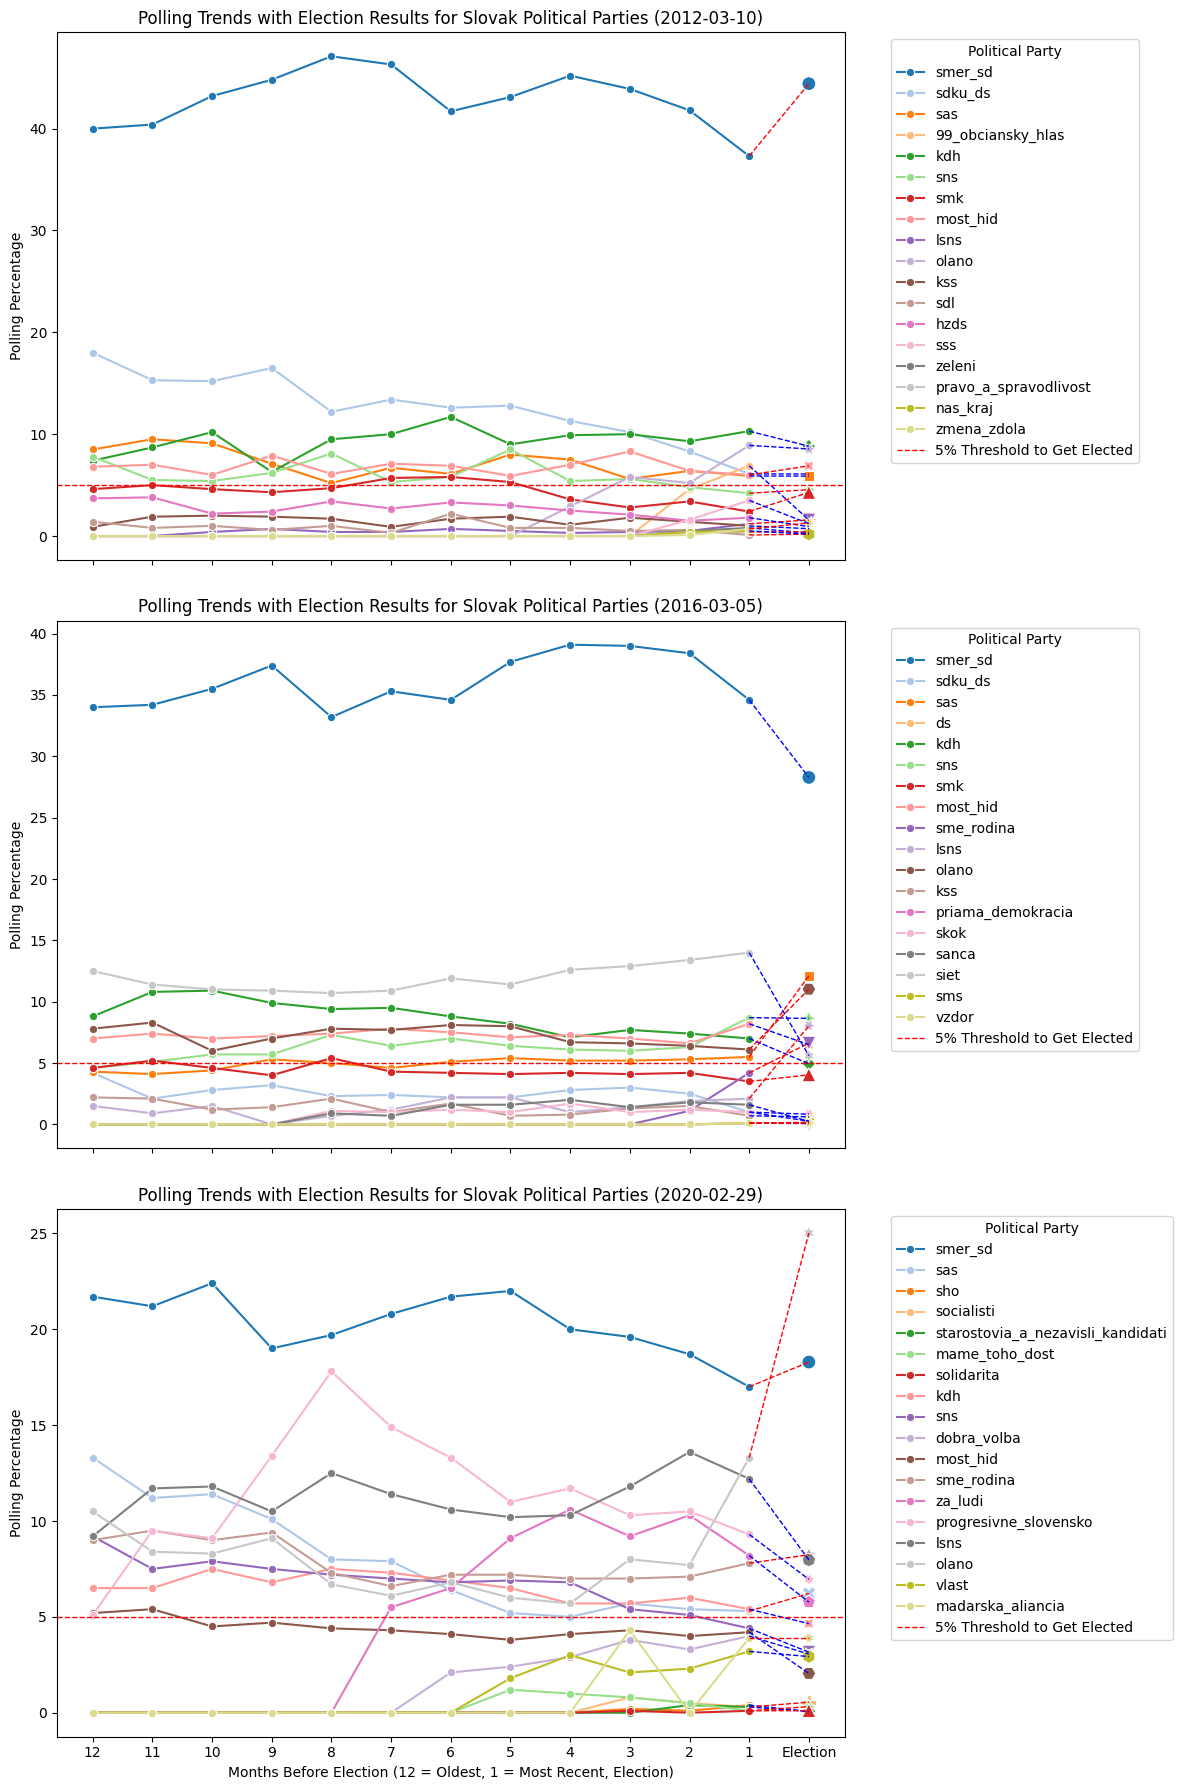
\includegraphics[width=\textwidth]{images_exploratory/Polls_with_result_ALL.png}
    \caption{}
\end{figure}

\newpage

Voľby v roku 2012 mali jasného favorita v strane SMER, ktorá po voľbách aj sama zostavila vládu, čo sa považuje za následok chaotického pádu vlady a následné predčasné voľby. Strana SDKÚ sa dramaticky prepadala v prieskumoch z 18\% rok pred voľbami, až na 6\% vo voľbách. 

Vo voľbách v roku 2016 už SMER stratil na sile a v posledných mesiacoch kampane utrpel prepad na 28\%. Zaujimavý vývoj mala strana Sieť, ktorá sa v prieskumoch dostávala nad 10\% celkom konzistentne, avšak v poslednom mesiaci kampane jej voliči pravdepodobne prestúpili k iným stranám ako OĽaNO, SaS či Sme rodina. Sieť sa tak prepadla až na hranicu zvoliteľnosti.

Voľby v roku 2020 sa ukazujú ako najvyrovnanejšie a to v tom zmysle, že viac strán dosahovalo v prieskumoch nad hranicu 10\%. Avšak ujať vedenia sa podarilo strane OĽaNO, ktorá rástla v posledných mesiacoch pred voľbami zatiaľ najvýraznejšie zo všetkých pozorovaných strán v prieskumoch, až ich aj nakoniec vyhrala. Graf nezachytáva realitu, toho že koalícii Progresívne Slovensko-Spolu sa nepodarilo dostať do parlamentu, keďže kandidovali ako koalicia dvoch strán a pre takýto typ politického subjektu je potrebné dosiahnuť vo voľbách viac ako 7\%. 

Trend toho, že vládne strany počas výkonu moci strácajú na podpore v následujúcich voľbach vyzerá ustálený v rámci všetkých volieb, ešte sa naň pozrieme bližšie. 

\subsection{Dopad predošleho vládnutia na voľby}

V našich dátach je informácia o tom či v predošlom volebnom období bola daná strana v parlamente a či bola súčasťou koalície/opozície. Bolo by teda vhodné sa pozrieť na to, ako sa menila voličská zakladňa strán v koalícii a strán, ktoré v nej neboli. 

\begin{figure}[!htbp]
    \centering
    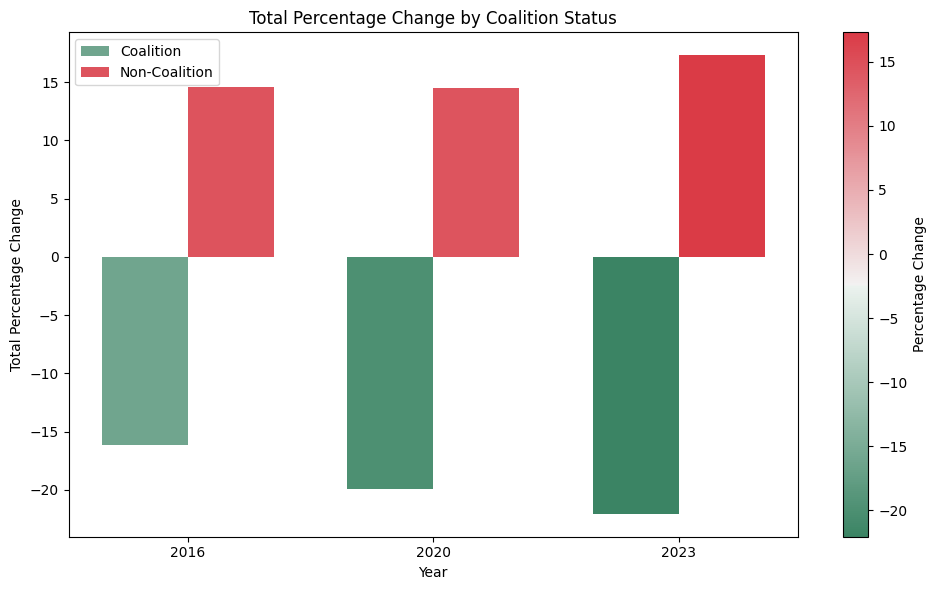
\includegraphics[width=\textwidth]{images_exploratory/Coalition_vs_NoCoalition.png}
    \caption{}
\end{figure}

V súčte strany vládnej moci vždy stratili až cez 15 percent v nasledujúcich voľbách, avšak miera straty nebola ustálená, teda chceme veriť, že kvalita vládnutia aspoň do nejakej miery ovplyvnila, koľko by dané strany stratili v následujúcich voľbách. V závislosti od tohto strany mimo vladnej koalície nabrali vo výsledkoch približne v rovnakom množstve. Rovnako volič mohol od vládnej koalicie prejsť k strane, ktorá má k nej blízko a po voľbách sa k nej pridala. Preto aj keď z roku 2012 na 2016 SMER stratil cez 15 percent tak komfortne zostavil vládu v roku 2016 za pomoci SNS, MOST - HÍD a Siete.

\subsection{Pohlaď na koaličné strany a rozvoj krajiny}

Po zistení z predchádzajúcich analýz, že sa stranám po spolupráci v koaličných vládach znižuje voličské zastúpenie, sme sa rozhodli preskúmať, či by tento jav nemohol byť zapríčinený ekonomicko-sociálnymi faktormi.
Po úprave našich datasetov, ktoré zachytávajú vývoj všeobecných faktorov krajiny, ako napríklad HDP, a datasetu spojeného so stranami, ich koaličnými partnermi a obdobiami ich vládnutia, sme zistili, že napriek pravidelným stratám vo voličskom zastúpení jednotlivých koaličných strán nevieme tento úpadok vidieť v trendoch rôznych štatistík o krajine.

Na grafoch nižšie je zobrazená koalícia a jej celé predošlé obdobie vládnutia. To znamená, že rozhodnutia koaličných strán z roku 2016 mali vplyv na vývoj situácie od roku 2012 až po 2016. Pri mnohých ukazovateľoch, ako je napríklad percento nezamestnanosti, sa podarilo udržať klesajúci trend. Rovnako sa podarilo udržať rastúci trend pri HDP a ďalších ukazovateľoch. V prípade situácie s klesajúcim rizikom chudoby sa tiež prevažne podarilo udržať klesajúci trend. Dá sa teda povedať, že rozhodnutie voličov prestať podporovať danú stranu nemusí byť vždy spôsobené negatívnymi rozhodnutiami strán, ale aj inými faktormi, ako sú napríklad vyjadrenia politikov či iné okolnosti. Avšak, nie je to pravidlom.  

\begin{figure}[H]
	\centering
	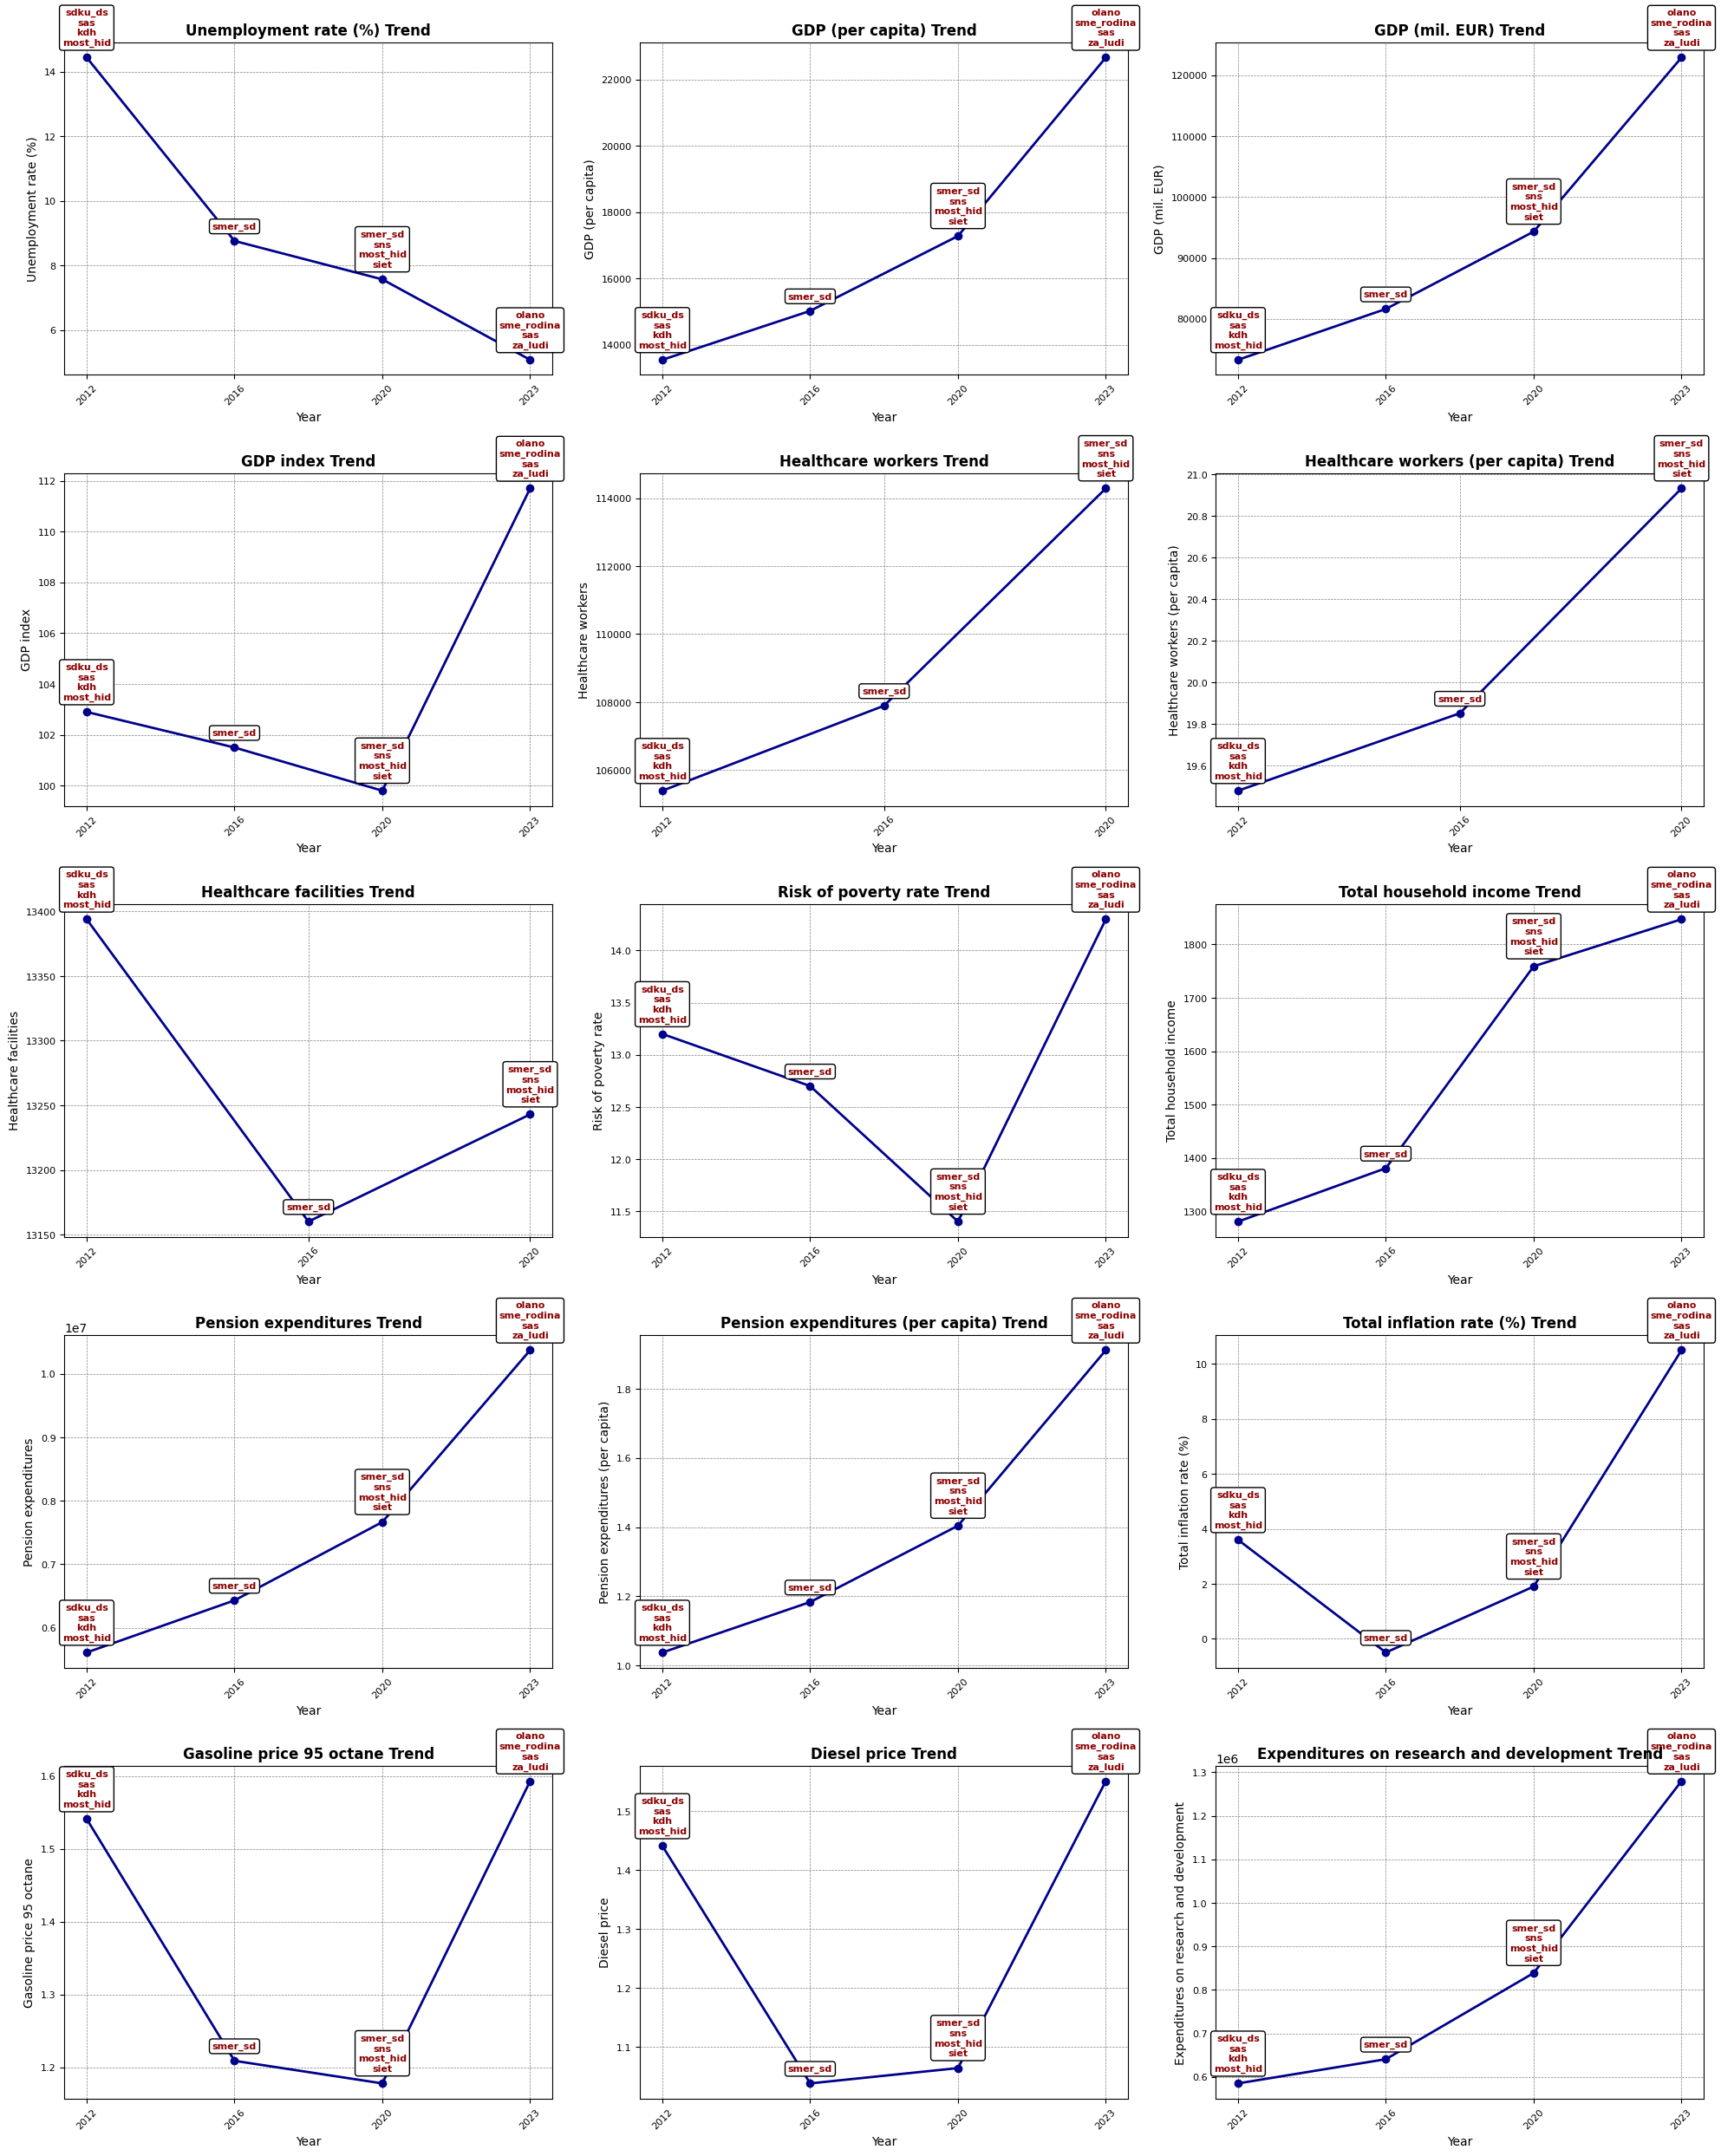
\includegraphics[width=0.98\textwidth]
	{images_exploratory/Coalition_Progress.png}
	\caption{}
\end{figure}

\newpage

Ďalším naším krokom bolo hlbšie sa zamerať na ideologické a štrukturálne faktory vládnucich koalícií a preskúmať, či ich spoločné hodnoty, ako je liberalizmus, orientácia na ľavú alebo pravú politickú stranu, postoj k integrácii do EÚ a ďalšie, zohrávali úlohu pri formovaní rastu krajiny. Porovnaním koalícií s rôznymi ideológiami sa snažíme zistiť, či tieto rozdiely ovplyvnili ich schopnosť podporovať pokrok v kľúčových oblastiach. 

Naše dáta boli získané z Politického kompasu, ktoré však nie vždy presne zodpovedajú dátam týkajúcim sa zvolených strán, keďže nie všetky strany boli zahrnuté v Politickom kompase.


\begin{figure}[!htbp]
    \centering
    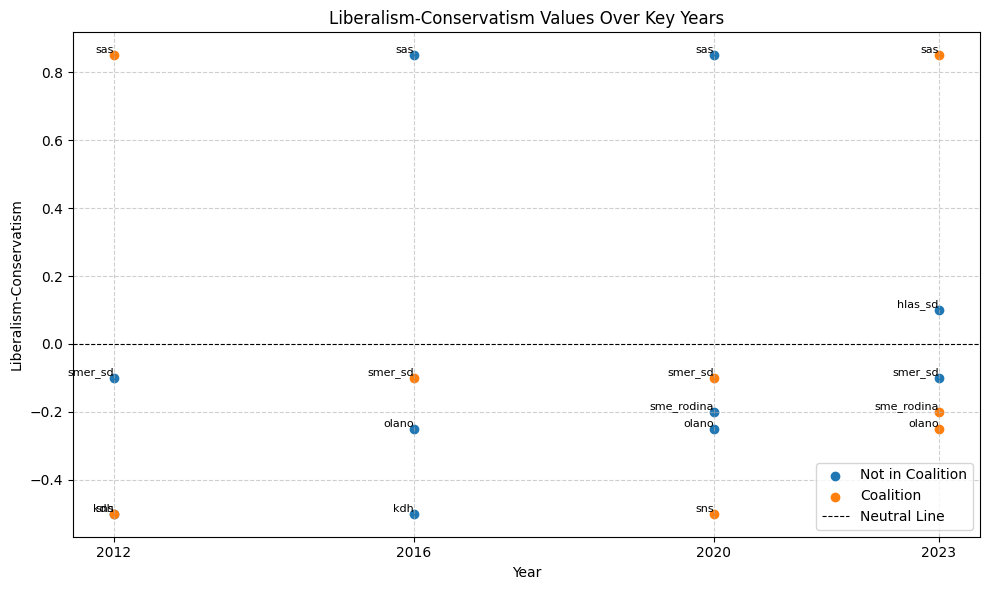
\includegraphics[width=\textwidth]
    {images_exploratory/Liberalism-Conservatism.png}
    \caption{}

    \centering
    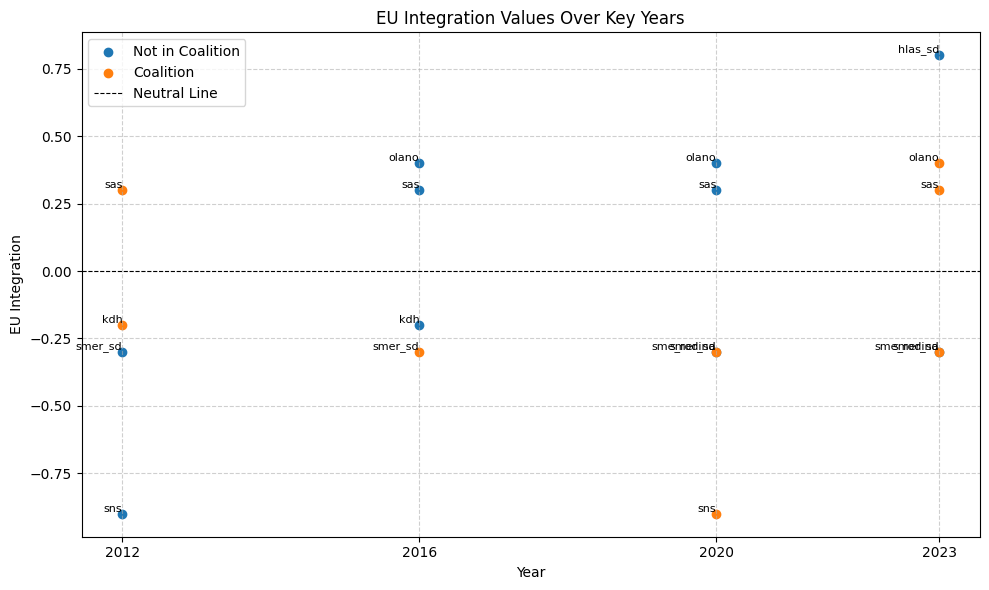
\includegraphics[width=\textwidth]
    {images_exploratory/EU-Intergration.png}
    \caption{}
\end{figure}

\clearpage
Ako si môžeme všimnúť napríklad v politickom období medzi rokmi 2020 a 2023, koalícia bola zložená zo strán SaS, OĽaNO, Sme rodina a Za ľudí. Hoci sa tieto politické subjekty líšia v otázkach integrácie do EÚ a v pozícii na škále liberalizmus – konzervativizmus, napriek tomu dokázali posilniť celkovú hospodársku situáciu v krajine. Výraznejšie napríklad narástlo HDP a zároveň sa podarilo znížiť mieru nezamestnanosti. Na druhej strane však nedošlo k žiadnemu výraznému zlepšeniu v oblasti inflácie a cien plynu, ktoré sa im počas tohto obdobia nepodarilo dostať pod kontrolu. Za niektoré nepriaznivé javy, ktoré sa im nepodarilo odstrániť, však nemusí niesť plnú zodpovednosť iba táto koalícia, keďže do vývoja zasiahli aj iné externé faktory a krízy.

\end{document}

